%!TEX program = xelatex
%%% template.tex
%%% This LaTeX source document can be used as the basis for your technical
%%% paper or abstract. Intentionally stripped of annotation, the parameters
%%% and commands should be adjusted for your particular paper - title,
%%% author, article DOI, etc.
%%% The accompanying ``template.annotated.tex'' provides copious annotation
%%% for the commands and parameters found in the source document. (The code
%%% is identical in ``template.tex'' and ``template.annotated.tex.'')

\documentclass[review]{acmsiggraph}


\TOGonlineid{Paper\_0000}
\TOGvolume{0}
\TOGnumber{0}
\TOGarticleDOI{1111111.2222222}
\TOGprojectURL{}
\TOGvideoURL{}
\TOGdataURL{}
\TOGcodeURL{}

\usepackage{graphics}
\usepackage{url}
\usepackage{hyperref}
\usepackage{subfigure}
\usepackage{algorithm}
\usepackage{algorithmic}
\usepackage{amsthm}
\usepackage{mathptmx}
\usepackage{amsmath,bm}
\usepackage{textcomp}
\usepackage{mathrsfs}
\usepackage{enumerate}
%%%Start for Chinese Setting
\usepackage{xeCJK}
\usepackage{fontspec}
\setCJKmainfont{SimSun}
\setmainfont{Times New Roman}
%%%End for Chinese Setting

\newcommand{\comment}[1]{}
\newcommand{\xj}[1]{\textcolor[rgb]{1.00,0.00,0.00}{(xuejin: #1)} }
\newcommand{\redemph}[1]{\textcolor[rgb]{1.00,0.00,0.00}{#1}}
\newcommand{\blueemph}[1]{\textcolor[rgb]{0.00,0.00,1.00}{#1}}
\newcommand{\vb}[1]{\mathbf{#1} }
\newcommand{\mathpo}[1]{\left( \begin{array}{c} x\\y \end{array} \right)}
\newcommand{\mathp}[2]{\left( \begin{array}{c} #1\\#2 \end{array} \right)}
\newcommand{\objmodel}{\mathbf{O}}
\newcommand{\tabincell}[2]{ \begin{tabular}{@{}#1@{}}#2\end{tabular} }
\newtheorem{theorem}{Theorem}



%\title{Behavior Analysis in Interior Scenes from Dynamic RGBD images }
\title{ Behavior Recovery/Analysis in Cluttered and Dynamic Indoor Scene  }

\author{Paper0000 }
\pdfauthor{Paper0000}

\keywords{Indoor scene, behavior analysis, dynamic, object correspondence}

\begin{document}

 \teaser{
 \includegraphics[width=2\columnwidth]{figures/teaser.png}
 \caption{Behavior recovery and behavior-based editing of dynamic cluttered indoor scenes.
 	From a set of dense scans at different times (a), our system first extract the object correspondences (b) and behavior model (\xj{optionally show a graph}). The recovered behavior model can be applied to many applications, such as scene editing (c) and indoor scene synthesis (d).}
  \label{fig:teaser}
 }

\maketitle

\begin{abstract}

While modeling static indoor scenes using RGBD cameras has been extensively studied in recent years, 
we introduce a \emph{behavior recovery} system to investigate the behavior of objects in an cluttered indoor scene.
%
In a daily indoor environment, because of object functions and human behaviors, the spatial placements of objects presents non-unique but statistically regular displacements.
%Behavior Analysis in Cluttered and Dynamic Indoor Scene
We take the \emph{inverse problem} to recover object behaviors from a collection of point clouds captured at different times in a dynamic indoor scene.
%
Our system consists of two key parts, \emph{extraction of object correspondence} and \emph{behavior model}. 
%
Given a collection of dense point clouds of an indoor scene in daily use at different times, the correspondence between objects are extracted using an iterative segmentation-and-registration process.
%
Our algorithm is robust to noise and incomplete parts in imperfect scans. 
%
In the second part is to recover object behaviors, which represent the spatial arrangement of objects and interrelations between objects. 
%
Using our method, the correlation between concrete geometry and semantic behaviors of an indoor scene can be established.  
Therefore, the recovered behavior model can be adopted to many applications that requires labeled 3D database, such as scene synthesis, scene arrangement and so on. 
%
%The spatial placements of objects at different times implicitly encode the object functions and human behavior in the environment.
%RGBD cameras is becoming more and more popular for common users to capture the environment where they live. 
% 
We evaluate our algorithm on a number of indoor scenes including office, bedroom and so on.
The results demonstrate that our algorithm build accurate object correspondence from imperfect scans of cluttered indoor scenes, based on which, the recovered behavior provides natural principles for many other applications oriented to indoor scenes. 



\end{abstract} 


\keywordlist 
\section{Introduction}
\label{sec:intro}
\mdf{In this paper, we present a new method to solve the object-level joint registration and co-segmentation problem. This problem originates from our attempt to build databases from scanned data.} \hsy{One reviewer said we should state this at the beginning of the introduction, he didn't understand our motivation until the late of introduction}
Many research projects and applications of indoor scenes require segmented, and even annotated 3D databases~\cite{SearchClassify,SceneFromExample,Fisher:2012:ESO:2366145.2366154,Chen:2014:ASM:2661229.2661239,Fisher:ActivityCentricSceneSynthesis}).
%
One way to build such a database is to interactively compose scenes using 3D object models, resulting in scenes with object segmentation and annotation naturally available, or to manually segment and annotate existing 3D scenes. 
%
This procedure can be tedious and time consuming, despite many efforts of improving the interaction experience~\cite{Merrell:2011:IFL:2010324.1964982, Xu:2013:SSC:2461912.2461968}.
%
Another way is to automatically generate scenes from 3D shape models according to images~\cite{Liu2015Model,Chen:2014:ASM:2661229.2661239}. 
%
In these methods, a retrieval procedure is usually needed and inevitably limit the result to a certain set of 3D models despite the actual 3D model in the input images.

Generating scene models directly from captured point clouds will significantly facilitate dataset construction and \mdf{increase} the dataset variety.
%
One of the major gaps between the required dataset and the available scene capturing frameworks~\cite{KinectFusion, dai2016bundlefusion} is the generic object-level segmentation. 
%
A generic object-level segmentation is not an equivalence of multi-label classification problem since it is not limited to a fixed number of objects in different scenes. 
%
Existing approaches for segmenting scanned 3D data require additional knowledge, such as the block-based stability~\cite{3DReasoningfromBlockstoStability}, or the motion consistency of rigid objects~\cite{Xu:2015:ACS:2816795.2818075}.  
%
%\cite{Xu:2015:ACS:2816795.2818075} proposes a practical and rather complete framework to close the gap between the required data set and available scene capturing method. 
%
%One of the observation in \cite{Xu:2015:ACS:2816795.2818075} is that the motion consistency of rigid object can serve as a strong evidence of general objectness.
While they employ a robot to do proactive push and use the movement tracking to verify and iteratively improve their object level segmentation result, \mdf{it remains significantly} challenging to recover the motion consistency in a \mdf{non-invasive} way.
\hsy{Without robot, our method is more tedious, since we need to schedule scanning every day.}


In this paper, we explore the motion consistency of rigid objects in a different aspect.
%
While the motion consistency of objects in indoor scenes is naturally revealed by human activities along the time, we hope to segment the objects in a scene from the scanned point clouds at different times. 
%
With respect to this idea, we are facing the choice of scanning schemes. 
%
One way is to record the change of the scene along with human activities.
Another option is to schedule a periodic sweep that only records the result of human activities but avoids the instants of human motion. 
%
The main challenge brought in by the second scheme is that we may not be able to solve the object correspondence by a local search due to the sparse sampling over time.
However, the very same challenge exists in the first scheme due to the occlusion caused by human bodies, not to mention other additional process (e.g. tracking with severe occlusions) needed for human bodies.
%
Therefore, we choose the second scheme.
\cxj{What is the advantage of the second scheme?} \hsy{Both schemes are difficult. We simply choose the less difficult one. The second scheme simply has less disadvantage.}
%
With the second scanning scheme, our original intention of building 3D scene datasets from canned data leads us to the problem of coupled joint registration and co-segmentation.


In this problem, registration and segmentation are entangled in each other. 
%
On one hand, the segmentation depends on the registration to connect the point clouds into series of rigid movement so that the object-level segmentation can be done based on the motion consistency. On the other hand, the registration depends on the segmentation to break the problem into a series of rigid joint registration instead of a joint registration with non-coherent point drift.
Non-coherent point drift means that a pair of points is close to each other in one point set, but their corresponding pair of points in another point set is far from each other. 
%
This happens when this pair of points actually belong to different objects.


We employ a group of Gaussian mixture models and each of these Gaussian mixture models represents a potential object. 
This model unentangle \cxj{Where do you find the word "unentangle"? did you create it?} \hsy{As verbs the difference between untangle and unentangle is that untangle is to remove tangles or knots while unentangle is to reverse the process of entanglement. Disentangle is to free something from entanglement.} the registration and segmentation in the way that the segmentation can be done by evaluate the probability of points belongs to the Gaussian mixture models and the registration can be done by evaluate rigid registration against each Gaussain mixture models.


In summary our work makes following contributions: 
\begin{enumerate}
	\item To the best of our knowledge, we first put forward the problem of joint registration and co-segmentation of point sets.
	
	\item We propose a generative model to simultaneously solve the joint registration and co-segmentation of point sets.
	
	\item We design a practical tool for efficient joint registration and co-segmentation based on the generative model. 
	
\end{enumerate}


\section{Related Work}
\label{sec:rw}
In this section we explain how our work is related to the previous work on point set processing and how we draw experiences from these methods. 

%\subsection{Point Set Registration with GMM Representation}
%\label{subsec:gmmreg}
\noindent{\textbf{Point Set Registration with GMM Representation.}}
There is a series of approaches that use Gaussian mixture model as \mdf{the} representation for point set registration problems \cxj{due to its general ability of representing point sets for both rigid and non-rigid registation}.
%
%
A \mdf{comprehensive} survey about approaches for point set registration using Gaussian mixture models can be found in \cite{GMM_PAMI}. 
They also present a unified framework for rigid and nonrigid registration problems. 
%
These methods select one of the point sets as the ``model'' and align other point sets with this \mdf{template}. \cxj{Is it better to use "template" than ``model''?} 
%
Myroeko and Song consider the registration of two point sets as a probability density estimation problem, and use Gaussian mixture model to represent the geometry and force the GMM centroids to move coherently as a group to preserve the topological structure of the point sets \cite{CPD}. This method is applicable to both rigid registration and non-rigid registration. \cxj{Does this method treat one point set as the template?}
%
As we highlighted in Sec.~\ref{sec:intro}, our problem is different from the non-rigid registration while the point drift is non-coherent in our \mdf{problem}.
%
Unlike these works, \cite{Evangelidis2014} treats all point sets equally.
They are all realizations of a Gaussian mixture model and the registration is cast into a clustering problem. 
A recent method pushes this idea to the application on a large scale dataset~\cite{GOGMA}. 
Comparing to these methods, our method can be seen as an extension of the formulation of \cite{Evangelidis2014} to simultaneously handle joint registration and co-segmentation. 
\cxj{It should not be a simple extension. You should highlight what is the most challeging part we solved compared with others. I would say: } \mdf{In comparison, we employ the same GMM representation of object models while we formulate the non-coherent point drift as .....  }

%\subsection{Image segmentation and co-segmentation}
%\label{subsec:coseg}
\noindent{\textbf{Image segmentation and co-segmentation}}
%
An influential work for interactive image segmentation is GrabCut~\cite{grabcut}. It uses two Gaussian mixture models, one for foreground and the other for background. 
To initialize these two Gaussian mixture models, a rectangle is manually placed to contain the foreground. 
Our design of interaction draws on the \mdf{experience} from \cite{grabcut}. 
%
The difference is that our interaction is designed for 3D space and can handle multi-object segmentation rather than foreground-background segmentation. 
%
\cite{Taniai_2016_CVPR} jointly recovers co-segmentation and dense per-pixel correspondences in two images. 
Its co-segmentation is limited to foreground-background segmentation. Our work solves a similar problem for multiple 3D point sets. 
\cxj{There are many image co-segmentation papers. If you want to discuss it, you should discuss more. }

\noindent{\textbf{Segmentation from Motion.}}
The idea that motion can be a strong hint for segmentation is used in many works.
\cite{Xu:2015:ACS:2816795.2818075} employs a robot to do proactive push and track the motion to learn object segmentation. 
\cite{unsupervisededge} exploits the motion in a video and uses the motion edges as the training data to learn an edge detector for image \cxj{use 'an image' or 'images'}. 
These methods lean on the motion that is continuous in time and can be tracked. Our method can handle motion that is not continuous in time.

\noindent{\textbf{3D Object Recognition based on Correspondence Grouping.}}
By allowing interactively input \mdf{the scene layout}, the joint registration and co-segmentation problem can be treated as a series of 3D object recognition problem in point sets. Our method should be classified as one of the correspondence grouping method. Comparing to previous methods \cxj{that uses ...}~\cite{hough,LOF}, our method simultaneously solve\mdf{s} the problem for multiple target models in multiple scenes.

\section{Overview}
\label{sec:overview}

\begin{figure*}
	\includegraphics[width=1.0\textwidth]{figures/overview}
	\caption{System overview.}
	\label{fig:overview}
\end{figure*}

The objective of our algorithm is to recover object behaviors from a set of point clouds scanned at different times for an indoor scene.
%
To achieve this goal, objects and correspondences between objects and point clouds must be extracted. 
%
More specifically, our problem is to transfer the noisy and incomplete point-level data into object-level models and correspondences to understand the object behaviors in the scene.
%


Our system consists of two main steps, \emph{point cloud segmentation} and \emph{object registration}, as Figure~\ref{fig:overview} shows. 
The \textbf{input} is a set of point clouds scanned using a RGBD camera (a). 
We scan each scene at different times \blueemph{during a month} using a Microsoft Kinect V1. A set of dense point clouds are generated using a real-time fusion system~\cite{NieBner:2013:VoxelHashing}. 
%
It is burdensome to scan every detailed structure in a cluttered indoor scene. As a result, each point cloud is incomplete and noisy due to object occlusions.



We first segment each frame simply using \blueemph{region growing} (b).
There are very likely many wrong boundaries in the generated patches.
Then we cluster all the patches from all frames into $k$ clusters using $k$means. 
%
\cite{Jia20153D} have demonstrated the power of features based on bounding box in the segmentation of indoor objects.
Therefore, we design the descriptor of each patch as the cascades of length, width and height of its bounding box, mean and standard deviation of the distance of each point to its bounding box, percentage of closest points to the faces of its bounding box.  
The feature dimension is then reduced using PCA. 
\xj{Currently, this step is manually done.} 



In each cluster, the patches are registered using a joint registration method~\cite{Evangelidis-ECCV-2014} to produce the object model of this cluster (c).
%
There are inevitably wrong registration due to wrong clustering. 
Therefore, we project the generated object models back into each frame using the estimated transformation. 
Re-segmentation is performed using the model consistency and neighborhood information in each frame, as described in Sec.~\ref{sec:segmentation}.
By iteratively register resegmented patches and re-segment frames, our system converges to a set of well-registered 3D object models and accurate correspondence between object model and all point clouds. 
%
Then we learn the behavior model (d) based the object correspondences from all input point clouds (Sec.~\ref{sec:behavior}), then apply the behavior model into many applications (Sec.~\ref{sec:applications}). 




\comment{
\begin{enumerate}
\item  \emph{Registration/Labeling:} Given a sequence of RGBD data captured in different times and views, we first register \emph{all the RGBD images} to segment objects and detect motions according to their low-rank characteristics using Robust PCA~\cite{candes2011robust}.
%
Given the assumption that there are typically static objects, such as wall, floor and so on, moving objects can be treated as sparse noise and the static backgrounds can be separated and completed as low-rank part by the robust PCA.
The point clouds are then divided into two categories: static objects and dynamic objects.
Combing the separated sparse part and the low-rank part, \emph{object segmentation} is performed by combing the motion, depth, and appearance features in the RGBD images. 

\comment{
\emph{Progressive Object Modeling} Static objects are reconstructed based on geometry primitives/model database. Dynamic objects are typically small size, connected with a large static object. They can be reconstructed by combing the point clouds captured under different views.
}
%\emph{Spatial Distribution:} After each round of registration and labeling of the input RGBD images, we can refine the spatial distribution map of each object. The map describes its position, poses and so on in the indoor environment. The interconnection between objects are then progressively refined.


\item \emph{Function Analysis/Behavior Map:}  
With the segmented regions, objects should be identified according to their appearance and geometry features among the entire image sets. 
We build a dynamic behavior map including all of the objects in the scene. Each node is an object/a part of an object. The edges in the graph describe the spatial relationship between objects/parts.
The object behavior can be explored from its surrounding objects in the dynamic structure graph. With a dynamic behavior map, the RGBD data is re-segmented and re-labeled to obtain semantical consistency of the scene.

\end{enumerate}
}
	

 








\section{Iterative Co-Segmentation and Joint Registration}
\label{sec:segmentation}
\begin{figure*}
	\includegraphics[width=1.0\textwidth]{figures/hsy/overview}
	\caption{Iterative co-segmentation and joint registration.}
	\label{fig:iterative-segmentation-registration}
\end{figure*}
\subsection{Region Grow}
\subsection{Object Clustering}
\subsection{Joint Registration}
\subsection{Global Consistent Graph Cut}
Figure~\ref{fig:object-iterations} shows the segmentation is progressively refined. 

\begin{figure*}
\centering
\includegraphics[width=2\columnwidth]{figures/object-iterations.png}
\caption{ The segmentation of each frame is progressively refined based on registered object models. From left to right: an input point cloud (a), segmentation updates at three iterations. \xj{show corresponding object model at each 
		iteration.} 	 }
\label{fig:object-iterations}
\end{figure*}

\section{Behavior Model}
\label{sec:behavior}


Our behavior model in a dynamic scene consists of three parts. 
One is the behavior of single object, which is represented by the statistics of the object motion (rotations/translations) interpreted from its orientations and positions in frames.
%
The second is the behavior of a group of object, which means the correlations of the statistics of the motions of objects. Their supporting/proximity relationship or arrangements of a group of objects keep consistent. 
%
c. The relationship variations caused by motion of the objects in the set of point clouds. In other words, the behavior of the object relationship. For example, the support relationship of vase can change from one desktop to another desktop or so.  

\comment{
\subsection{Static Object Relations}

The static object relations are defined in two-level. The first level is the pairwise relation between any two objects, supporting and proximity. The second is the structural group which describes the spatial distribution of a subset consisting of more than two objects, such as symmetric or uniformly distributed objects.

\subsubsection{Pairwise Object Relations}
}
\subsection{Pairwise Object Relations}
\label{sec:pairwise_relation}


In a cluttered indoor scene, there are many pairs of objects that usually co-occur in the scene with some typical geometric relations in a long time period. 
%
In our system, we consider two types of pairwise relations, which are commonly used to describe object relations in many previous methods~\cite{Fisherscenesynth12,Silberman:ECCV12,Xu13sig,xu_sig14}.


\paragraph{Support} $SR(\objmodel_a,\objmodel_b)$ indicates that $\objmodel_a$ is supported by $\objmodel_b$. We use a Gaussian function to indicate the distribution of $\objmodel_a$ on the supporting surface of $\objmodel_b$;
%
In each frame, we check any pair of objects connected by a surface. 
Typically, smaller object is supported by the larger one, the upper object is supported by the bottom object.
%
%We scale the supported $\objmodel_b$ into a unit square with factor $s_x,s_y$, then scale
We transform the object been supported $\objmodel_a$ into the local coordinates of its support object $\objmodel_b$ to get its location $\mathbf{x}_a$ and orientation $\theta_a$.
%
According to all the examples of this pair in the input frames, we compute a Gaussian function
\begin{equation}
	\label{eq:sr_ab}
	SR(\objmodel_a,\objmodel_b) = \mathcal{N}_{position}(\mathbf{\mu}_{x},\Sigma_{x}) \mathcal{N}_{orientation}(\mu_{o},\sigma_{o})
\end{equation} 
Each relation has a confidence or frequency $w$ in all the frames. 




\paragraph{Proximity} $PR(\objmodel_a,\objmodel_b)$ indicates $\objmodel_a$ is close to $\objmodel_b$ in with a Gaussian function $\mathcal{N}(\mu,\sigma)$ including position $x,y$ in the local coordinate system of $\objmodel_a$ and the orientation $\theta_b$ of $\objmodel$  in the local coordinate system of $\objmodel_b$, defined as 
%\xj{only considering object pairs that are close enough, say $dis(o_a,o_b)<Thr_{proximity}$?} 
%
\begin{equation}
	\label{eq:proximity_ab}
	PR(\objmodel_a,\objmodel_b) = \mathcal{N}_{position}(\mathbf{\mu}_{x},\Sigma_{x}) \mathcal{N}_{orientation}(\mu_{o},\sigma_{o}).
\end{equation} 



If the background floor and wall are taken into account for pairwise relations, the relation between a single object and the background is actually the behavior of this object itself.




\subsection{Group Behavior}
\label{sec:groupbehavior}

Based on all the extracted pairwise relation, a directed graph $G(V,E)$ is constructed to encode the mutual relations of all the objects in the scene, as shown in Figure~\ref{fig:geometric_graph}. 
Each node is an object model in the scene.   
%
Each directed edge represents a pairwise geometric relation between two objects. 
%
The information carried in each edge includes:
\begin{enumerate}
	\item \textbf{Relation type}:  supporting or proximity. Each edge is directed from a small object to an larger object indicating that the small object is usually associated with a larger object. 
	%
	\item \textbf{Edge weight}: is the frequency of that two objects co-occur in the scene. We define it 
	\begin{equation}
		w(i\to j)= \frac{c(i\to j)}{K}	\end{equation}
	where $c(i\to j)$ is the total counts of that two objects co-occur and follow the relation defined by the edge in all the frames. $K$ is the number of all frames.
	\comment{Note: if there is only one frame where a cup is placed on a cabinet while it is always placed on an office desk, there will be a supporting edge from the cup to the cabinet but with very low weight. Do we remove this weak edge using threshold? This truncation can be done in the reliable group selection as well.}
	
	\item \textbf{Relation description}: Associated with each edge, the statistics of the spatial relations defined in Sec.~\ref{sec:pairwise_relation} is also stored. 
\end{enumerate}



%\subsubsection{Structural Group}
%\label{sec:group-relation}

A \textbf{structural group} $G_s$ is defined as a \emph{complete graph} in which every pair of nodes in connected by a unique edge, to describe the mutual relations between nodes in a subset.
%\xj{The completeness of a structural group guaranttees the compactness of each subgroup. } 
%
From the directed graph $G(V,E)$, a set of structural groups can be extracted. There are many potential structural groups in $G$. The smallest structural group is an edge connecting two nodes. 
%with a reliability $\rho_{sg}$. 
%
However, we only focus on reliable structural groups for further application, such as layout re-arrangement, unusual event detection, etc. 
%
The reliability of a structural group $G_s(V_s,E_s)$ with $k$ objects is defined as defined as
\begin{equation}
	\label{eq:reliability_sg}
	\rho_{sg} = \big(\prod_{e_i \in E_s} {w(e_i)}\big)^{\frac{1}{k}}
\end{equation}



\begin{figure}
	\centering
	\includegraphics[width=0.98\columnwidth]{figures/geometric_graph.png}
	\caption{Construction a directed geometric graph from pairwise relations. Green edges indicate supporting relations. Purple edges represent proximity relations. The edge width indicates the frequency of each relation. Each dashed ellipse represents a structural group. \redemph{The pair (B,C) should be very weak because they are far away from other other, and can be removed. Otherwise, (A,B,C) is another structural group.}}
	\label{fig:geometric_graph}
\end{figure}


\comment{
\paragraph{Multiple instances}
%

\xj{More explaination of multiple instances.}
%
When there are multiple instances of the same object model co-occur in an indoor scene, for example, two chairs with a table, as shown in Figure~\ref{fig:multiple_instance_sg}, the two instances are registered to the same object model in the segmentation and registration step. 
%
In the construction of the geometric graph, each node is an object model. So the two chairs are represented as the one node B, as shown in Figure~\ref{fig:multiple_instance_sg}(b). The pairwise relation between the table and the chair is proximity, with the spatial relation can be modeled by \redemph{two Gaussians}. 

However, this representation implicitly discards the behavior relations between the objects of the same type. 
Moreover, the geometric graph could not exactly reflect the layout of the target scene.            
\xj{If two instances are treated as two distince nodes, how to recover the correspondences between frames?}    

We introduce the another type of structural group $G_{mi}$, as shown in Figure~\ref{fig:multiple_instance_sg}(c).
A structural group with multiple instances have the following properties:
\begin{enumerate}
	\item The structural group have more than one object instances which are registered to the same geometry model. 
	\item The multiple instances having the same geometric relation with the same host object. For example, two chairs must always close to the same desk in the scene, or two boxes are supported by the same table.
\end{enumerate}

\xj{Not all instances follow this definition. Only the instances following these properties compose a structural group, as Figure~\ref{fig:multiple_instance_a} shows.}


For a structural group with multiple instances, the geometric relation of each instance with its supporting object is computed as following:
\begin{enumerate}
	\item For an object model, find all the frames where multiple instances co-occur. 
	\item Find the same host object to all of the instances. 
	\item In the local coordinate system of the host object, map the positions and orientations of all the instances. 
	\item If $k$ instances co-occur in the scene, then recover a GMM model with $K$ Gaussians for the $k$ instances.  
\end{enumerate}

\begin{figure}
	\centering
	\includegraphics[width=\columnwidth]{figures/instance_graph_2.png}
	\caption{A structural group with multiple instances co-occur in the scene.}
	\label{fig:multiple_instance_sg}
\end{figure}


\begin{figure}
	\centering
	\includegraphics[width=\columnwidth]{figures/instance_graph_3.png}
	\caption{Not all instances should be described using structural graph with multiple instances. (a) The two lamps can be represented using one node (A), which are separately supported by two other objects (B and C). (b) If the two instances are highly correlated, it is much better to clearly represent their spatial relations using two distinct nodes (A1, A2). }
	\label{fig:multiple_instance_a}
\end{figure}

}


\comment{
	\begin{algorithm}
		\caption{Behavior analysis given object registration}
		\label{alg:behavior}
		\begin{algorithmic}[1]
			\State {Input: A set of RGBD patches $\patch_{i,k}$, $k=1,\ldots,K$ frames.}
			\State {Input: A set of object models $\objmodel_{i}$, $i=1,\ldots,M$.}
			\State {Input: correspondence between each patch and object models $\patch_i = \mathbf{T}_i\objmodel_j$.} 
			\State {Compute the \emph{supporting relations} between any pair of object models $SR(\objmodel_i,\objmodel_j)$;}
			\State {Compute the \emph{proximty relations} between any pair of patches $PX(\objmodel_i,\objmodel_j)$;}
			\State {Build a directed graph $G(V,E)$ consisting of all the objects in the scene.}
			\State {Extract structural group from $G(V,E)$ with high reliability: $\rho_{sg} > T_{sg}$.}
			\State {Extract structural group with multiple instances. }
			
		\end{algorithmic}
	\end{algorithm}
}








\input{applications.tex}
\section{Results and Discussions}
\label{sec:results}
\section{Conclusions}
In this paper, we present 



\bibliographystyle{acmsiggraph}
\bibliography{indoorRef}
\end{document}
